\documentclass{beamer}
\usepackage[utf8]{inputenc}

\usetheme{Madrid}
\usecolortheme{default}
\usepackage{amsmath,amssymb,amsfonts,amsthm}
\usepackage{mathtools}
\usepackage{txfonts}
\usepackage{tkz-euclide}
\usepackage{listings}
\usepackage{adjustbox}
\usepackage{array}
\usepackage{gensymb}
\usepackage{tabularx}
\usepackage{gvv}
\usepackage{lmodern}
\usepackage{circuitikz}
\usepackage{tikz}
\lstset{literate={·}{{$\cdot$}}1 {λ}{{$\lambda$}}1 {→}{{$\to$}}1}
\usepackage{graphicx}

\setbeamertemplate{page number in head/foot}[totalframenumber]

\usepackage{tcolorbox}
\tcbuselibrary{minted,breakable,xparse,skins}



\definecolor{bg}{gray}{0.95}
\DeclareTCBListing{mintedbox}{O{}m!O{}}{%
  breakable=true,
  listing engine=minted,
  listing only,
  minted language=#2,
  minted style=default,
  minted options={%
    linenos,
    gobble=0,
    breaklines=true,
    breakafter=,,
    fontsize=\small,
    numbersep=8pt,
    #1},
  boxsep=0pt,
  left skip=0pt,
  right skip=0pt,
  left=25pt,
  right=0pt,
  top=3pt,
  bottom=3pt,
  arc=5pt,
  leftrule=0pt,
  rightrule=0pt,
  bottomrule=2pt,
  toprule=2pt,
  colback=bg,
  colframe=orange!70,
  enhanced,
  overlay={%
    \begin{tcbclipinterior}
    \fill[orange!20!white] (frame.south west) rectangle ([xshift=20pt]frame.north west);
    \end{tcbclipinterior}},
  #3,
}
\lstset{
    language=C,
    basicstyle=\ttfamily\small,
    keywordstyle=\color{blue},
    stringstyle=\color{orange},
    commentstyle=\color{green!60!black},
    numbers=left,
    numberstyle=\tiny\color{gray},
    breaklines=true,
    showstringspaces=false,
}
%------------------------------------------------------------
%This block of code defines the information to appear in the
%Title page
\title %optional
{4.11.5}
\date{15 September, 2025}
%\subtitle{A short story}

\author % (optional)
{INDHIRESH S - EE25BTECH11027}

\begin{document}

\frame{\titlepage}

\begin{frame}{Question}
 Find the equation of the plane passing through the points $(2, 5, -3)$, $(-2, -3, 5)$, and $(5, 3, -3)$. Also, find the point of intersection of this plane with the line passing through points $(3, 1, 5)$ and $(-1, -3, -1)$.
\end{frame}

\begin{frame}[allowframebreaks] 
\frametitle{Equation}
    \centering
    \label{tab:parameters}
Let the given points be:
\begin{align}
   \Vec{A}=\myvec{2\\5\\-3}\;,\Vec{B}=\myvec{-2\\-3\\5}\;and\;\Vec{C}=\myvec{5\\3\\-3}
\end{align}
\end{frame}

\begin{frame}
\frametitle{Theoretical Solution}
For equation of plane:
\begin{align}
   \myvec{\Vec{A}&\Vec{B}&\Vec{C}}^T\Vec{n}=\myvec{1\\1\\1}
\end{align}
\begin{align}
   \myvec{2&-2&5\\5&-3&3\\-3&5&-3}^T\Vec{n}=\myvec{1\\1\\1}
\end{align}
\begin{align}
   \myvec{2 & 5 & -3\\-2 & -3 & 5\\5 & 3 & -3}\Vec{n}=\myvec{1\\1\\1} \Rightarrow \augvec{3}{1}{2 & 5 & -3&1\\-2 & -3 & 5&1\\5 & 3& -3&1}
\end{align}
\end{frame}

\begin{frame}
\frametitle{Theoretical solution}
\begin{align}
   \augvec{3}{1}{2 & 5 & -3&1\\-2 & -3 & 5&1\\5 & 3& -3&1}\xleftrightarrow[R_2\longleftarrow R_2+R_1]{R_3\longleftarrow R_3-\frac{5}{2}R_1}  \augvec{3}{1}{2 & 5 & -3&1\\0 & 2 & 2&2\\0 & \frac{-19}{2}& \frac{9}{2}&\frac{-3}{2}}
\end{align}
\begin{align}
     \augvec{3}{1}{2 & 5 & -3&1\\0 & 2 & 2&2\\0 & \frac{-19}{2}& \frac{9}{2}&\frac{-3}{2}} \xleftrightarrow{R_2\longleftarrow\frac{1}{2}R_2} \augvec{3}{1}{2 & 5 & -3&1\\0 & 1 & 1&1\\0 & \frac{-19}{2}& \frac{9}{2}&\frac{-3}{2}}
\end{align}
\begin{align}
   \augvec{3}{1}{2 & 5 & -3&1\\0 & 1 & 1&1\\0 & \frac{-19}{2}& \frac{9}{2}&\frac{-3}{2}} \xleftrightarrow{R_3\longleftarrow R_3+\frac{19}{2}R_2} \augvec{3}{1}{2 & 5 & -3&1\\0 & 1 & 1&1\\0 & 0& 14&8}
\end{align}
\end{frame}

\begin{frame}
\frametitle{Theoretical Solution}
\begin{align}
     \augvec{3}{1}{2 & 5 & -3&1\\0 & 1 & 1&1\\0 & 0& 14&8} \xleftrightarrow{R_3\longleftarrow\frac{R_3}{14}}\augvec{3}{1}{2 & 5 & -3&1\\0 & 1 & 1&1\\0 & 0& 1&\frac{4}{7}}
\end{align}
\begin{align}
    \augvec{3}{1}{2 & 5 & -3&1\\0 & 1 & 1&1\\0 & 0& 1&\frac{4}{7}}\xleftrightarrow[R_2\longleftarrow R_2-R_3]{R_1\longleftarrow R_1+3R_3} \augvec{3}{1}{2 & 5 & 0&\frac{19}{7}\\0 & 1 &0 &\frac{3}{7}\\0 & 0& 1&\frac{4}{7}}
\end{align}
\begin{align}
    \augvec{3}{1}{2 & 5 & 0&\frac{19}{7}\\0 & 1 &0 &\frac{3}{7}\\0 & 0& 1&\frac{4}{7}}\xleftrightarrow{R_1\longleftarrow R_1-5R_2}  \augvec{3}{1}{2 & 0 & 0&\frac{4}{7}\\0 & 1 &0 &\frac{3}{7}\\0 & 0& 1&\frac{4}{7}}
\end{align}
\begin{align}
     \augvec{3}{1}{2 & 0 & 0&\frac{4}{7}\\0 & 1 &0 &\frac{3}{7}\\0 & 0& 1&\frac{4}{7}}\xleftrightarrow{R_1\longleftarrow \frac{R_1}{2}}\augvec{3}{1}{1 & 0 & 0&\frac{2}{7}\\0 & 1 &0 &\frac{3}{7}\\0 & 0& 1&\frac{4}{7}}
\end{align}
\end{frame}

\begin{frame}
\frametitle{Theoretical Solution}

The equation of plane can be given as:

\begin{align}
\Vec{n}^T\Vec{x}=c
  \end{align}
Therefore the equation of plane can be given as
\begin{align}
  \myvec{2\\3\\4}^T\Vec{x}=7
\end{align}
  
Where
\begin{align}
    n=\myvec{2\\3\\4}\;\;and\;\; c=7
\end{align}
\end{frame}

\begin{frame}
\frametitle{Theoretical Solution}

The equation of line passing through the points $(3,1,5)$ and $(-1,-3,-1)$
\begin{align}
    \Vec{x}=\Vec{h}+k\Vec{m}
\end{align}
Multiply with $\Vec{n^T}$ on both sides:
\begin{align}
    \Vec{n^T}\Vec{x}=\Vec{n^T}\Vec{h}+k\Vec{n^T}\Vec{m}
\end{align}
From Eq.12
\begin{align}
    c=\Vec{n^T}\Vec{h}+k\Vec{n^T}\Vec{m}
\end{align}
\begin{align}
   \frac{ c-\Vec{n^T}\Vec{h}}{\Vec{n^T}\Vec{m}}=k
\end{align}
\begin{align}
    \Vec{m}=\myvec{3-(-1)\\1-(-3)\\5-(-1)}
\end{align}

\end{frame}

\begin{frame}
\frametitle{Theoretical Solution}
  \begin{align}
     \Vec{m}=\myvec{4\\4\\6}
\end{align}
Now substitute the corresponding values in Eq.18
\begin{align}
   \frac{7-\myvec{2\\3\\4}^T\myvec{3\\1\\5}}{\myvec{2\\3\\4}^T\myvec{4\\4\\6}}=k
\end{align}
\begin{align}
    \frac{7-29}{44}=k
\end{align}


\end{frame}

\begin{frame}
\frametitle{Theoretical Solution}
   Solving this we get
\begin{align}
k=\frac{-1}{2}
\end{align}
Now substitute the value of k in Eq.15
\begin{align}
    \Vec{x}=\myvec{3-2\\1-2\\5-3}
\end{align}
Therefore the point of intersection is:
\begin{align}
    \Vec{x}=\myvec{1\\-1\\2}
\end{align}
\end{frame}

\begin{frame}[fragile]
    \frametitle{C Code}
    \begin{lstlisting}
#include <stdio.h>

void solve(double *out) {
    int A[3] = {2, 5, -3};
    int B[3] = {-2, -3, 5};
    int C[3] = {5, 3, -3};
    int P[3] = {3, 1, 5};
    int Q[3] = {-1, -3, -1};

    // vectors
    int AB[3] = {B[0]-A[0], B[1]-A[1], B[2]-A[2]};
    int AC[3] = {C[0]-A[0], C[1]-A[1], C[2]-A[2]};

    // normal = AB x AC
    int n[3];
    n[0] = AB[1]*AC[2] - AB[2]*AC[1];
    n[1] = AB[2]*AC[0] - AB[0]*AC[2];
    n[2] = AB[0]*AC[1] - AB[1]*AC[0];
    int d = -(n[0]*A[0] + n[1]*A[1] + n[2]*A[2]);
    \end{lstlisting}
\end{frame}

\begin{frame}[fragile]
    \frametitle{C Code}
    \begin{lstlisting}
   // direction of PQ
    int v[3] = {Q[0]-P[0], Q[1]-P[1], Q[2]-P[2]};
    int num = -(n[0]*P[0] + n[1]*P[1] + n[2]*P[2] + d);
    int den = n[0]*v[0] + n[1]*v[1] + n[2]*v[2];

    double t = (double)num / den;
    double X = P[0] + t*v[0];
    double Y = P[1] + t*v[1];
    double Z = P[2] + t*v[2];
    \end{lstlisting}
\end{frame}

\begin{frame}[fragile]
    \frametitle{C Code}
    \begin{lstlisting}
   // output: n0, n1, n2, d, X, Y, Z
    out[0] = n[0];
    out[1] = n[1];
    out[2] = n[2];
    out[3] = d;
    out[4] = X;
    out[5] = Y;
    out[6] = Z;
}
    \end{lstlisting}
\end{frame}

\begin{frame}[fragile]
    \frametitle{Python Code}
    \begin{lstlisting}
import ctypes
import numpy as np
import matplotlib.pyplot as plt
from mpl_toolkits.mplot3d import Axes3D

# Load the shared library
lib = ctypes.CDLL("./intersection.so") # use "plane.dll" on Windows

# Prepare output buffer (7 doubles)
out = (ctypes.c_double * 7)()
lib.solve(out)

# Extract results
n = [out[0], out[1], out[2], out[3]]
intersection = [out[4], out[5], out[6]]
    \end{lstlisting}
\end{frame}

\begin{frame}[fragile]
    \frametitle{Python Code}
    \begin{lstlisting}
print(f"Equation of plane: {n[0]}x + {n[1]}y + {n[2]}z + {n[3]} = 0")
print(f"Intersection point: {intersection}")

# --- Plotting ---
A = np.array([2,5,-3])
B = np.array([-2,-3,5])
C = np.array([5,3,-3])
P = np.array([3,1,5])
Q = np.array([-1,-3,-1])
I = np.array(intersection)

fig = plt.figure()
ax = fig.add_subplot(111, projection="3d")

# Plot the plane
xx, yy = np.meshgrid(range(-2,7), range(-4,7))
zz = (-n[0]*xx - n[1]*yy - n[3]) / n[2]
    \end{lstlisting}
\end{frame}

\begin{frame}[fragile]
    \frametitle{Python Code}
    \begin{lstlisting}
ax.plot_surface(xx, yy, zz, alpha=0.3, color="cyan")

# Plot line PQ
t_vals = np.linspace(-1,2,20)
linePQ = np.array([P + t*(Q-P) for t in t_vals])
ax.plot(linePQ[:,0], linePQ[:,1], linePQ[:,2], "g", label="Line PQ")

# Plot points
ax.scatter(*A, color="r", s=50, label="A(2,5,-3)")
ax.scatter(*B, color="b", s=50, label="B(-2,-3,5)")
ax.scatter(*C, color="m", s=50, label="C(5,3,-3)")
ax.scatter(*I, color="k", s=80, marker="o", label="Intersection F(1,-1,2)")
ax.text(2, 5, -3, "A", color="red", fontsize=12)
ax.text(-2, -3, 5, "B", color="blue", fontsize=12)
ax.text(5, 3, -3, "C", color="purple", fontsize=12)
ax.text(1, -1, 2, "F", color="black", fontsize=12)
    \end{lstlisting}
\end{frame}

\begin{frame}[fragile]
    \frametitle{Python Code}
    \begin{lstlisting}
ax.set_xlabel("X-axis")
ax.set_ylabel("Y-axis")
ax.set_zlabel("Z-axis")
ax.legend()
plt.savefig("./figure1.png")
plt.show()
    \end{lstlisting}
\end{frame}

\begin{frame}{Plot}
    \begin{center}
        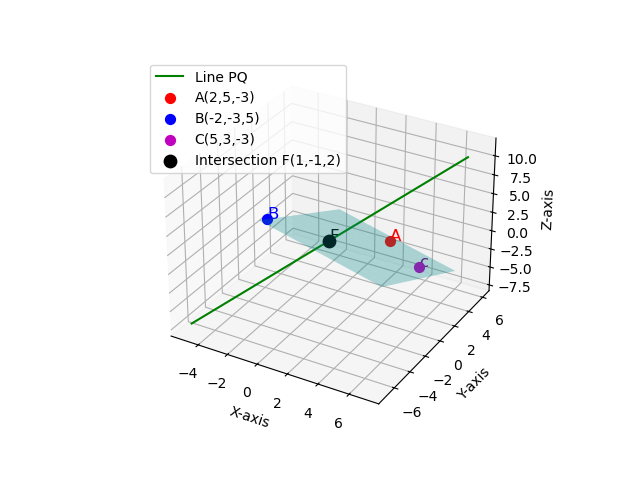
\includegraphics[width=\columnwidth, height=0.8\textheight, keepaspectratio]{figs/figure1.png}
    \end{center}
\end{frame}

\end{document}